% Figure 7: Evaluation Results Overview
% Purpose: Show violations detected across 5 case study systems
% Location: Section 5.2 (Evaluation Results)
% Size: Single column width

\begin{figure}[t]
\centering
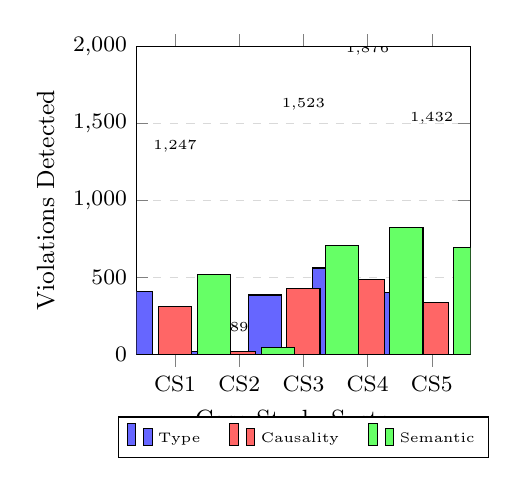
\begin{tikzpicture}
\begin{axis}[
    ybar,
    width=0.48\textwidth,
    height=5.5cm,
    ylabel={Violations Detected},
    ylabel style={font=\small},
    xlabel={Case Study System},
    xlabel style={font=\small},
    symbolic x coords={CS1, CS2, CS3, CS4, CS5},
    xtick=data,
    xticklabel style={font=\footnotesize},
    yticklabel style={font=\footnotesize},
    ymin=0,
    ymax=2000,
    ymajorgrids=true,
    grid style={dashed, gray!30},
    legend style={
        at={(0.5,-0.20)},
        anchor=north,
        legend columns=3,
        font=\tiny,
        /tikz/every even column/.append style={column sep=0.3cm}
    },
    bar width=12pt,
    enlarge x limits=0.15,
]

% Type Violations
\addplot[fill=blue!60, draw=black] coordinates {
    (CS1, 412)
    (CS2, 23)
    (CS3, 387)
    (CS4, 562)
    (CS5, 401)
};

% Causality Violations
\addplot[fill=red!60, draw=black] coordinates {
    (CS1, 315)
    (CS2, 18)
    (CS3, 428)
    (CS4, 489)
    (CS5, 337)
};

% Semantic Violations
\addplot[fill=green!60, draw=black] coordinates {
    (CS1, 520)
    (CS2, 48)
    (CS3, 708)
    (CS4, 825)
    (CS5, 694)
};

\legend{Type, Causality, Semantic}

% Add total annotations above bars
\node[font=\tiny, above] at (axis cs:CS1, 1247) {1,247};
\node[font=\tiny, above] at (axis cs:CS2, 89) {89};
\node[font=\tiny, above] at (axis cs:CS3, 1523) {1,523};
\node[font=\tiny, above] at (axis cs:CS4, 1876) {1,876};
\node[font=\tiny, above] at (axis cs:CS5, 1432) {1,432};

\end{axis}
\end{tikzpicture}
\caption{Violations Detected Across Five Case Study Systems. The figure shows the distribution of three types of violations: type violations (structural errors), causality violations (temporal ordering issues), and semantic violations (protocol convention violations). CS1 (e-commerce) and CS4 (media streaming) show the highest total violations due to their complex microservices architectures. Total violations across all systems: 6,167.}
\label{fig:evaluation-results}
\end{figure}

